\documentclass[11pt]{article}
\usepackage{graphicx}
\usepackage{amssymb}
\usepackage{amsmath}



\usepackage[html,dvipsnames]{xcolor}


\setlength{\textwidth}{6.5in}
\setlength{\textheight}{9.0in}
\headheight=0.5in
\topmargin=-0.75in
\oddsidemargin= 0.0in
\evensidemargin=-0.25in


\usepackage[pdfauthor={Brandon Franzke},pdftitle={EE 599 Project Summary},% 
    pdftex,bookmarks]{hyperref}
\hypersetup{colorlinks,% 
    citecolor=green,%
    filecolor=Orange,%
    linkcolor=blue,%
    urlcolor=BrickRed,%
    pdftex}



\pagestyle{myheadings}
\markright{{\bf EE 541 - \copyright B. Franzke - Fall 2021} }


\title{\bf {\small EE 541 -- Computational Introduction to Deep Learning} \\ Initial Project Proposal}
\author{\copyright Prithvi Anandkumar Dalal, Shoumik Nandi, Aditya Anulekh Mantri}

\begin{document}
    \maketitle

    \paragraph{Project Title:}  Using GANs to create Monet Styled Paintings from Photos

    \paragraph{Project Team:} Prithvi Anandkumar Dalal, Shoumik Nandi, Aditya Anulekh Mantri

    \paragraph{Competition summary:}
    For this project we propose to create a model to segment neuronal cells in light-microscopy images.
    We will build a model to delineate objects and cells of interest common in biological images of neurological disorders (Figure \ref{fig:nseg}).
    Neuronal cell segmentation is a critical first step to quantify how neurological disorders respond to treatment.
    Current computer vision solutions are a poor-fit becase neuronal cells have a unique, irregular, and concave morphology that differs from other cellular mask heads.
    A successful model will use the training phase contrast microscopy images to segment neuronal instances in noveal images with a high level of accuracy.

    \begin{figure}[!htb]
        \begin{center}
            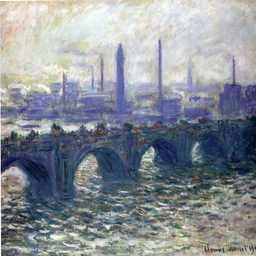
\includegraphics[width=0.3\linewidth]{images/3b262c6726}
            \caption{The generated images should look similar to the Monet painting shown above}
            \label{fig:nseg}
        \end{center}
        \vspace{-0.6cm}
    \end{figure}

    \paragraph{Competition page:}
    \href
    {https://www.kaggle.com/c/gan-getting-started/}
    {https://www.kaggle.com/c/gan-getting-started/}

    \paragraph{Competition data:}
    The competition dataset is 385.87 MB.
    It consists of 300 Monet styled paintings and 7028 photos.
    Each image has 3 channels and is 256x256 pixels.
    The dataset also includes .tfrecord files of the same images.
    We are supposed to submit 7000-10000 Monet styled images to the competetion.

    Submissions are evaluated on MiFID (Memorization-informed Fréchet Inception Distance), which is a modification from Fréchet Inception Distance (FID).

    In FID, we use the Inception network to extract features from an intermediate layer.
    Then we model the data distribution for these features using a multivariate Gaussian distribution with mean $\mu$ and covariance $\Sigma$.
    The FID between the real images  and generated images  is computed as:

    \begin{displaymath}
        \text{FID} = ||\mu_r - \mu_g||^2 + \text{Tr} (\Sigma_r + \Sigma_g - 2 (\Sigma_r \Sigma_g)^{1/2})
    \end{displaymath}
    Where $Tr$ represents the trace of the matrix.

    More information about the evaluation of the competetion can be found here \href{https://www.kaggle.com/c/gan-getting-started/overview/evaluation}{here}

    \paragraph{Primary References and Codebase:}  We propose to build on the approach used in

    \begin{itemize}

        \item Zhu, Jun-Yan & Park, Taesung & Isola, Phillip & Efros, Alexei. (2017). "\href{https://arxiv.org/pdf/1703.10593.pdf}{Unpaired Image-to-Image Translation Using Cycle-Consistent Adversarial Networks}" 2242-2251. 10.1109/ICCV.2017.244.

        \item Radford, Alec & Metz, Luke & Chintala, Soumith. (2016). "\href{https://arxiv.org/pdf/1511.06434.pdf}{Unsupervised Representation Learning with Deep Convolutional Generative Adversarial Networks.}"

        \item Blog post: \href{https://pytorch.org/tutorials/beginner/dcgan_faces_tutorial.html#implementation}{DCGAN Tutorial}

        \item Github codebases:
        \begin{itemize}
            \item \href{https://github.com/junyanz/pytorch-CycleGAN-and-pix2pix}{CycleGAN and pix2pix in PyTorch},
        \end{itemize}
    \end{itemize}


    \paragraph{Architecture Investigation Plan:}  We plan to first implement the U-net architecture described the above reference [Ronneberger2015] and apply our traning data.  We then will compare the results to a Mask R-CNN architecuture which often performs well with only minimal transfer learning [Durkee2021].  Neuronal microscopy images do not have directionality and we will make heavy use of data augmentation increase the relative size of our dataset.

    \paragraph{Estimated Compute Needs:}  Based on the data set size in the above paper and the benchmarks in this \href{https://lambdalabs.com/blog/titan-v-deep-learning-benchmarks/}{Lambda Labs Blog}, we estimate that one training run for our initial U-net architecture will take 14 hours on a single nVidia V100 GPU, which is the GPU resource in the AWS p3.2xlarge instance.  With spot pricing, which is roughly \$1 per hour, we expect \$15 per training run.  The proposed Mask R-CNN architecture will be roughly twice the complexity, so we estimation \$30 per run.  We expect to do a number of provisional runs to tune hyper-parameters.  We estimate that this will cost approximate \$40.  In addition, we expect to do approximately 4 full runs which brings our total estimated computing cost to roughly \$200.  Pooling our AWS promo resources, we expect to be about \$ 80 short of this value.

    \paragraph{Team Roles:} The following is the rough breakdown of roles and responsibilities we plan for our team:
    \begin{itemize}
        \item Prithvi Anandkumar Dalal: Data collection and cleaning, video production.  Code Mask R-CNN.
        \item Shoumik Nandi: Get existing U-net codebase running on an AWS instance.
        \item Aditya Anulekh Mantri: Data Augmentation and team-code Mask R-CNN, assist with U-Net.
    \end{itemize}
    All team members will work on the final report and video.

% #TODO
%    Competition Summary
%    Architecture Investigation Plan
%    Estimated Compute Needs
%    Team Roles
\end{document}